%\newpage
\section{Evidence for Chiral Anomaly in Na$_3$Bi}
\label{sec:na3bi:chiral}

In this section, we discuss our evidence for the chiral anomaly effect in Na$_3$Bi. We will demonstrate the negative longitudinal magnetoresistance(LMR) data of two Na$_3$Bi samples, and compare them with the theoretical predictions. Besides, we will discuss the unexpected results obtained and their possible reasons. Also, to compare with the MR data of Na$_3$Bi, we will present the resistivity and conductivity tensors in a tilted $\bf B$ for a conventional one-band anisotropic metal. We will show why the conventional transport theory deviates from our observations. Additionally, we will calculate the splitting magnitudes of the Weyl nodes as we discussed in above sections. At the end, we explain why the negative MR in our Na$_3$Bi samples cannot arise from localization. All these evidences suggest the chiral anomaly origin of the negative LMR in our samples.


\subsection{Negative Longitudinal Magnetoresistance in Na$_3$Bi}

Besides the above type of Na$_3$Bi with a high carrier density, we have also grown some Na$_3$Bi crystals with a much lower Fermi energy $E_F$. The crystals were grown in a similar way as we described above, but were annealed for ten weeks before opening the growth tube. The samples are also contacted and sealed in a plastic cell inside the argon glovebox before being loaded into the magnet, as discussed in the chapter ``Experimental Setup''. As shown in Fig.\ref{figWeyl}B, C, the $\rho$ v.s. $T$ profile displays a non-metallic behavior and the Hall effect indicates a low $n$-type carrier density $n\sim 1\times 10^{17}$ cm$^{-3}$. The Fermi wavevector that corresponds to this carrier density is $k_F = 0.013 \;\rm{\AA}^{-1}$ ($8\times$ smaller than $k_D$). The saturation of resistivity below 10 K indicates the dominance of electrons in the conductance, and the mobility we obtain is $\mu\sim$ 2,600 cm$^2$/(Vs). Due to the zero gap feature of 3D Dirac semimetals, the holes in the valence band are copiously excited even at low $T$. As a result, the Hall coefficient $R_H$ shown in Fig. \ref{figWeyl}C is $n$-type at low temperatures but changes sign above 62K. We could also estimate $E_F$ using the maximum in $R_H$ at 105 K, and it yields a $E_F\sim 3k_BT\sim$ 30 meV. 
%The unusual profiles of $\rho$ and the Hall coefficient $R_H$ in Fig.\ref{figWeyl}C imply the zero-$B$ energy spectrum shown in Fig.\ref{figWeyl}B. 

\begin{figure}[!htbp]
  \begin{center}
\includegraphics[width=1\linewidth]{ch-na3bi/figures/FigWeylRhoHall.pdf}
\caption{\label{figWeyl} 
(Panel A) Sketch of the Landau levels in a Weyl semimetal showing chiral states in the lowest LL with opposite velocities and chiralities (arrows)
$\parallel\bf B$. An $\bf E$-field $\parallel \bf B$ breaks chiral symmetry and leads to an axial current. 
Panel B shows the Fermi energy $\epsilon_F$ and the density of states $D(\varepsilon)$ in zero $B$ (bold curve). 
$f(\varepsilon)$ is the Fermi-Dirac distribution at 3 K and at $\sim$100 K. The inset shows the triangle anomaly that dictates the decay of the neutral pion $\pi^0$ into 2 photons $\gamma$. 
(Panel C) The $T$ dependence of the resistivity $\rho$ in $B=0$ and Hall coefficient $R_H$ in Na$_3$Bi.
$R_H$ is measured in $B<$2 T applied $\parallel \bf c$. At 3 K, $R_H$ corresponds to a density $n = 1.04\times 10^{17}$ cm$^{-3}$.  
The excitation of holes in the valence band leads to a sign change in $R_H$ near 70 K and a steep decrease in $\rho$. The inset shows the contact labels and the $x$ and $y$ axes fixed to the sample. 
(Panel D) Curves of the longitudinal magnetoresistance $\rho_{xx}(B,T)$ at selected $T$ from 4.5 to 300 K measured with $\bf B\parallel \hat{x}$ and $I$ applied to (1,4). The steep decrease in $\rho_{xx}(B,T)$ at 4.5 K reflects the onset of the axial current in the lowest LL. As $T$ increases, the occupation of higher LLs in conduction and valence bands overwhelms the anomalous term.
}
  \end{center}
\end{figure}

Analysis of the observed Shubnikov de Haas (SdH) oscillations (see below) in magnetoresistance also confirms the value of $E_F$ in our Na$_3$Bi samples. Fig. \ref{figSdH}A displays the clear SdH oscillations with a small frequency (a smooth background has been subtracted from the raw data) when $\bf B$ is aligned towards $\bf c$ . Through locating the index field $B_n$ as the extrema of the SdH oscillations, we obtain the Landau index plot in Fig.\ref{figSdH}B. A linear fitting to the index plot yields a FS cross section $S_F$= 4.8$\pm$ 0.3 T, corresponding to $E_F = 29\pm 2$ mV which is in a good agreement with the value from $R_H$. The SdH period also implies that $E_F$ enters the $N$ = 0 LL at $B$ = 6-8 T. 





The density inferred from $S_F$ ($n_e = 1.4\times 10^{17}$ cm$^{-3}$) is slightly higher than $n_H$. We also notice that there is some deviation from the straight line in Fig. \ref{figSdH}B, which may be explained by a $g$-factor of $\sim$20, comparable to that in Cd$_3$As$_2$observed~\cite{Jeon2014} by scanning tunneling microcsopy ($g^*\sim$ 40). Such a low $E_F$ suggests that the transport property of the 3D Dirac fermions in Na$_3$Bi crystals can be influenced more significantly by the splitting of Weyl nodes and the resulted charge pumping effect between the nodes. Therefore, this type of Na$_3$Bi crystals provides us a great opportunity to investigate the chiral anomaly effect predicted for Weyl fermions.


\begin{figure}[!htbp]
  \begin{center}
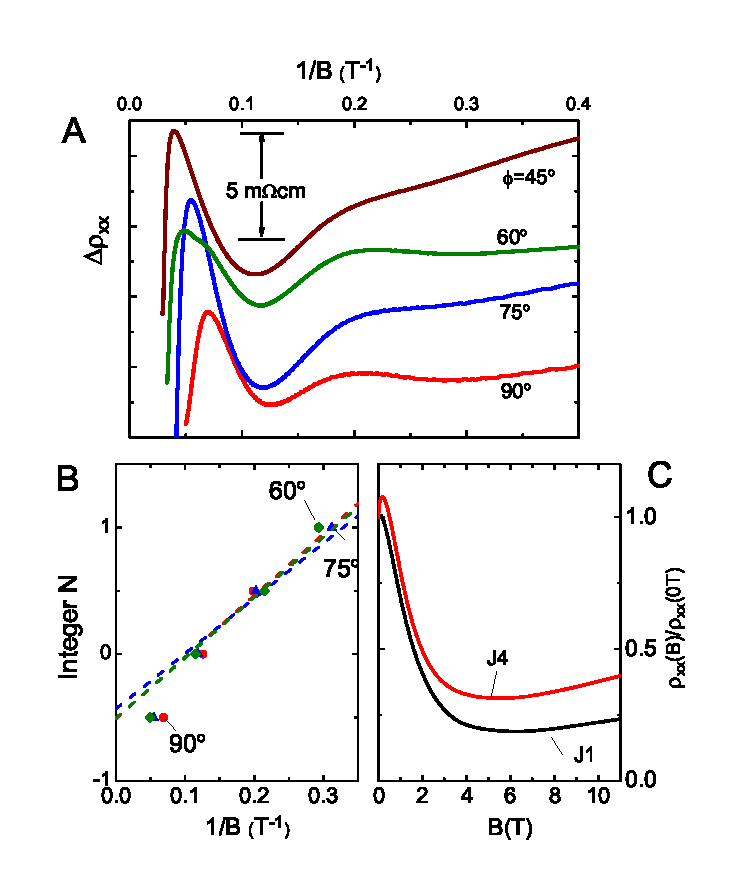
\includegraphics[width=0.9\linewidth]{ch-na3bi/figures/FigSdHMR}
\caption{\label{figSdH}
Panel A shows the Shubnikov oscillations resolved in $\rho_{xx}$ for several tilt angles $\theta$ (relative to $\bf \hat{x}$) after subtraction of the positive $B$-linear MR background (vertical scale as shown). The slope of the plot of the Landau level index $N$ vs. $1/B_n$ where $B_n$ locates the extrema of the oscillations yields $S_F$ = 4.8$\pm$ 0.3 T, $k_F$ = 0.013 $\rm{\AA}^{-1}$, and $E_F$ = 29$\pm$2 mV.  The deviation at large $B$ is consistent with a large $g^*\; (\sim 20)$. The field profiles of of $\rho_{xx}$ (inferred from $R_{14,23}$) in Sample J1 and J4, with $\bf B\parallel I$. The $N =0$ LL is entered at $B$= 6-8 T. The slight increase for $B>$ 5 T reflects the narrow width of the axial current. A slight misalignment of $\bf B$ (the uncertainty here is $\pm 1^\circ$) allows the $B$-linear positive MR component to appear as a background at large $B$. 
}
  \end{center}
\end{figure}


The 3D Dirac semimetals, Na$_3$Bi and Cd$_3$As$_2$~\cite{Wang2012,Wang2013}, comprise two Dirac cones located at opposite positions in the Brillouin Zone (Fig. \ref{figWeyl}A). Ref.~\cite{Wang2012} has provided detailed calculations to show that each Dirac cone could be separated into both left- and right-handed (Weyl) states that do not mix~\cite{Burkov2011,Yang2011, Aji2012,Son2013,Parameswaran2014,Hosur2013} when the time-reversal symmetry (TRS) is broken by the magnetic field. Besides, an axial current that flows between the paired Weyl nodes could be induced while both $\bf E$ and $\bf B$ are present, and it results in the negative longitudinal magnetoresistance in the semiclassical region as Son et.al.~\cite{Son2013} point out. Triggered by the above predictions, many experimental groups recently reported their negative MR results in different semimetals, such as  Bi$_{1-x}$Sb$_x$~\cite{Kim2013}, Cd$_3$As$_2$~\cite{Liang2015,Zhang2015a}, ZrTe$_5$~\cite{Li2014} and TaAs~\cite{Zhang2015}. However, we need to be cautious before reaching any conclusion because such negative MR exists in semimetals that are not Dirac or Weyl materials (e.g. Cd$_x$Hg$_{1-x}$Te~\cite{HgTe} and PdCoO$_2$~\cite{Kikugawa2014}). Thus it is important to identify a unique feature that could only be explained by the charge pumping effect and distinguishes the chiral anomaly from other effects in crystals. Below we will discuss a unique negative MR signature in Na$_3$Bi. We find that the enhanced conductance has a narrow plume shape whose direction is locked to the direction of $\bf B$. The enhancement steered by $\bf B$ suggests that it originates from the $\bf E\cdot \bf B$ pumping term.




%The intriguing possibility of observing the chiral (or axial) anomaly as a novel charge current in a crystal has been discussed since 1983~\cite{Nielsen}. In the field of topological phases of matter, this question has lately received intense interest in the context of Weyl semimetals~\cite{Ashvin,Balents,Son,Sid,Hosur}. [The anomaly first appeared as the dominant channel for the decay of the neutral pion into 2 photons $\pi^0\to 2\gamma$ (the Adler-Bell-Jackiw anomaly~\cite{Adler,Bell}). Subsequently, it has served broadly as a no-go test for the renormalizability of chiral gauge theories~\cite{Peskin,Zee}.]  To realize a Weyl semimetal, a promising path is to start with a 3D Dirac semimetal~\cite{Young,Bernevig}, and then split each Dirac node into a pair of Weyl nodes using a magnetic field $\bf B$. Rapid progress in identifying candidates for Dirac semimetals has been made~\cite{Young,Bernevig,Wang1,Wang2,Nagaosa}. The two semimetals specifically identified~\cite{Wang1,Wang2}, Na$_3$Bi and Cd$_3$As$_2$, were recently confirmed to be so by angle-resolved photoemission (ARPES)~\cite{Chen,Borisenko,Neupane,Liu,Suyang} and scanning tunneling microscopy~\cite{Yazdani}. Here we report the detection of the axial current in Na$_3$Bi as a highly collimated beam locked to the direction of $\bf B$.

A magnetic field $\bf B$ could split each Dirac node into two Weyl nodes with opposite chiralities $\chi=\pm 1$~\cite{Hosur2013,Wang2012} respectively. These Weyl nodes may be regarded as monopole sources and sinks of Berry curvature in $\bf k$ space. The Landau levels formed by these states are shown in Fig. \ref{figWeyl}B. One important feature in the LLs is that the lowest LL has a strict linear dispersion. And the chirality, which describes the handedness of the fermions, will determine whether the velocity is directed to the left or to the right. Therefore, it provides a solid-state platform to study the charge-pumping effect between fermions with different chiralities. In the absence of an electric field $\bf E$, the two chiral populations are separately conserved (Fig. \ref{figWeyl}A). However, application of $\bf E$ ruins the conservation and leads to a charge-pumping process between nodes, corresponding to the chiral anomaly sketched in Fig. \ref{figWeyl}B~\cite{Nielsen1983,Wan2011,Burkov2011,Son2013,Parameswaran2014,Hosur2013}. In a combination of $\bf E$ and $\bf B$, the electrons' charge-pumping rate between the two chiral branches is
\be
W = \chi\frac{e^3}{4\pi^2\hbar^2} {\bf E\cdot B},
\label{eq:W}
\ee
which is the direct result of the chiral anomaly effect~\cite{Burkov2011,Yang2011, Aji2012,Son2013,Parameswaran2014,Hosur2013}. When $\bf E$ and $\bf B$ are parallel, the pumping rate reaches the maximum, while the rate vanishes when $\bf E \perp \bf B$. Ideally, such pumping effect generates a longitudinal (axial) current. However, different from high energy physics, the charge pumping effect in a crystal is relaxed by the intervalley scattering. A relaxation time approximation describes the scattering rate as $1/\tau_v = CeB/\hbar v$, i.e. proportional to the LL degeneracy~\cite{Aji2012}. As a result, in the quantum limit, although the pumping rate becomes larger as the $B$ increases, the increment of the scattering rate counteracts that of the pumping rate. Thus the conductivity $\sigma_\chi\sim W\tau_v$ becomes independent of $B$ in the quantum limit. When many LLs are occupied, the axial current remains observable although reduced. In the semiclassical weak-$B$ limit, Son and Spivak~\cite{Son2013} show that
\be
\sigma_{\chi} = \frac{e^2}{4\pi^2\hbar c}\frac{v}{c}\frac{(eBv)^2}{E_F^2}\tau_v.
\label{eq:SS}
\ee
In contrast to the quantum limit case, the field dependence of $\sigma_\chi$ follows a quadratic behavior instead of a constant. Hence, the whole field picture of $\sigma_\chi$ has a $B^2$ growth at weak fields and a $B$-independent saturation in the quantum limit.

%%%%%%%%%%%
%As mentioned, the breaking of the time-reversal symmetry (TRS) by $\bf B$ causes each Dirac node to split into two Weyl nodes~\cite{Fang2012,Wang2012,Wang2013}. The Weyl nodes, which may be regarded as monopole sources and sinks of Berry curvature in $\bf k$ space, come in pairs with opposite chiralities $\chi=\pm 1$. In the absence of an electric field $\bf E$, the two chiral populations are separately conserved (Fig. \ref{figWeyl}A). However, application of $\bf E$ ruins the conservation and leads to a charge-pumping process between nodes, corresponding to the chiral anomaly sketched in Fig. \ref{figWeyl}B~\cite{Nielsen1983,Wan2011,Burkov2011,Son2013,Parameswaran2014,Hosur2013}. As shown in Fig. \ref{figWeyl}A, the lowest Landau level (LL) of the Weyl states in a crystal is chiral. For $\chi = 1$ the lowest LL is right-moving (velocity $\bf v\parallel \bf {B}$), whereas for $\chi=-1$ it is left-moving~\cite{Nielsen1983,Wan2011,Burkov2011,Son2013,Hosur2013}. At steady state, $\bf E$ transfers charge from say the $\chi = -1$ branch to the $\chi= 1$ branch at the rate below:~\cite{Hosur2013}
%\be
%W = \chi\frac{e^3}{4\pi^2\hbar^2} {\bf E\cdot B}.
%\label{eq:W}
%\ee
%The rate peaks for $\bf E\parallel B$ and vanishes when $\bf E\perp B$. In the weak-$B$ limit, a Berry curvature approach gives the chiral conductivity~\cite{Son2013} 
%\be
%\sigma_{\chi} = \frac{e^2}{4\pi^2\hbar c}\frac{v}{c}\frac{(eBv)^2}{\epsilon_F^2}\tau_v,
%\label{eq:SS}
%\ee
%where $\tau_v$ is the intervalley life-time and $\epsilon_F$ the Fermi energy. 

%The Dirac semimetal Na$_3$Bi grows as mm-sized, deep-purple, plate-like crystals with the largest face parallel to the $a$-$b$ plane ($\bf \hat{c}$ is normal to the planes). We annealed the crystals for 10 weeks before opening the growth tube~\cite{Satya}. To avoid oxidation, crystals were contacted using silver epoxy  in an Argon glove box, and then immersed in paratone in a capsule before rapid cooling. In Na$_3$Bi, the Dirac nodes are located at the wave vectors $(0,0, \pm k_D)$ with $k_D \simeq 0.1\; \mathrm{\AA}^{-1}$~\cite{Chen,Suyang}. The predicted existence of surface Fermi arcs was recently confirmed~\cite{HasanFS}. Initial experiments in our lab~\cite{Xiong} on samples with a large Fermi energy $\epsilon_F$ (400 mV) showed only a positive MR with the anomalous $B$-linear profile reported in Cd$_3$As$_2$~\cite{Liang}. 
%
%
%In a field $\bf B||\hat{z}$, each Dirac node divides into two Weyl nodes of chirality $\chi=\pm 1$~\cite{Hosur,Wang1}. As shown in Fig. \ref{figWeyl}B, the states are quantized into LLs. Specific to Weyl states, however, the lowest LL ($N$=0) has a constant slope, with velocity directed either to the left or to the right, depending on $\chi$. This dichotomy is the crystal analog of the left and right-handed populations~\cite{Nielsen}. Application of $\bf E\parallel \bf B$ leads to charge-pumping of electrons between the two branches at the rate
%\be
%W = \chi\frac{e^3}{4\pi^2\hbar^2} {\bf E\cdot B},
%\label{eq:W}
%\ee
%which expresses the chiral anomaly~\cite{Nielsen,Ashvin,Balents,Ran,Aji,Son,Sid,Hosur}. In the presence of impurities, the longitudinal (axial) current relaxes via an intervalley scattering rate given by $1/\tau_v = CeB/\hbar v$, i.e. proportional to the LL degeneracy~\cite{Aji}. Hence, the chiral conductivity $\sigma_\chi\sim W\tau_v$ is independent of $B$ in the quantum limit. We emphasize that, when many LLs are occupied, the axial current remains observable although reduced. In the weak-$B$ limit and when $\bf E$ and $\bf B$ are parallel, Son and Spivak~\cite{Son} show that
%\be
%\sigma_{\chi} = \frac{e^2}{4\pi^2\hbar c}\frac{v}{c}\frac{(eBv)^2}{E_F^2}\tau_v.
%\label{eq:SS}
%\ee
%As $B$ increases, $\sigma_\chi$ grows as $B^2$, but saturates to a $B$-independent value in the quantum limit.



We have seen such a B dependence in the longitudinal magnetoresistance of our Na$_3$Bi samples when $\bf B\parallel\hat{x}\parallel E $. As shown in Fig. \ref{figWeyl}D, the resistivity $\rho_{xx}$ displays a large negative LMR ($\bf B\parallel\hat{x}\parallel I $, the current) at low temperatures. The resistance measured is $R_{14,23}$ (defined in Fig. \ref{figWeyl}C, inset and caption). $\rho_{xx}$ has a peak around $B=0$ T, and then has a sharp decrease until it becomes nearly field independent at higher fields. The peak is suppressed as $T$ increases above $\sim$100 K (Fig. {figWeyl}D). In Fig. \ref{figSdH}C, the saturation of $\rho_{xx}$ (in Sample J1 and J4) happens above 5 T (the slight upturn at higher fields is a hint that the axial current is sensitive to misalignment of $\bf B$ at the level $\pm 1^{\circ}$). It is unexpected to see such a large negative LMR in a conventional conductor, even with band anisotropy (see below).

Then we hope to test whether this anomalous negative LMR arises from the chiral anomaly effect. Since the charge pumping rate is determined by the $\bf E\cdot \bf B$ term, it reaches the maximum when $\bf B$ is aligned with $\bf E$. We notice that the pumping rate only depends on the relative direction of $\bf E$ and $\bf B$ and does not care about the physical direction of them, when the field strengths are fixed. Thus a crucial test then is the demonstration that, the negative magnetoresistance (MR) pattern remains the same if $\bf E$ is rotated by 90$^\circ$. If it does, the axial current maximum is meant to be locked to $\bf B$ and $\bf E$, rather than being pinned to the crystal axes, even for weak $B$. Besides, we also need to test whether the axial current becomes smaller when $\bf B$ deviates from the direction of $\bf E$ with $\bf E$ fixed.

\begin{figure}[!htbp]
  \begin{center}
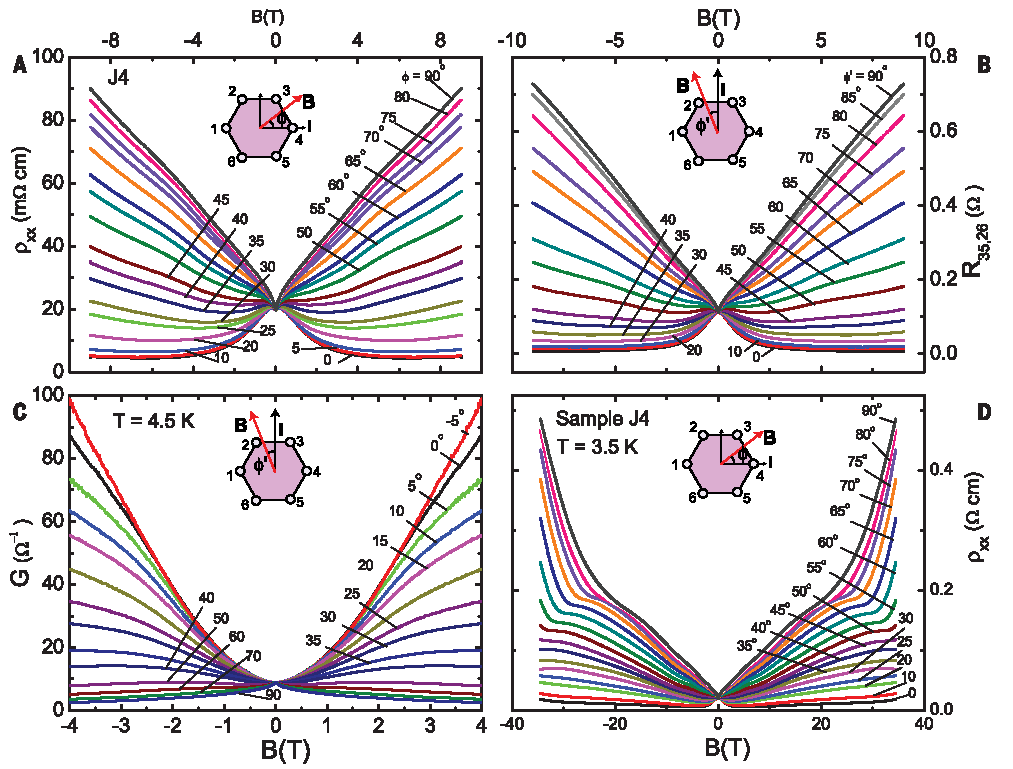
\includegraphics[width=1\linewidth]{ch-na3bi/figures/FigMR4.pdf}
\caption{\label{figMR4}
Evidence for axial current in Na$_3$Bi (J4) obtained from transport measurements in an in-plane field $\bf B$. Panel A shows plots of the resistivity $\rho_{xx}$ vs. $B$ at selected field angles $\phi$ to the $x$-axis (inferred from resistance $R_{14,23}$, see inset). For $\phi$ = 90$^\circ$, $\rho_{xx}$ displays a $B$-linear positive MR. However, as $\phi\to 0^\circ$ ($\bf B||\hat{x}$), $\rho_{xx}$ is strongly suppressed. Panel B shows plots of $R_{35,26}$ with $\bf E$ rotated by 90$^\circ$ relative to Panel A ($\bf B$ makes angle $\phi'$ relative to $\bf\hat{y}$; see inset). The resistance $R_{35,26}$ changes from a positive MR to negative as $\phi'\to 0^\circ$. In both configurations, the negative MR appears only when $\bf B$ is aligned with $\bf E$. Panel C shows the conductance $G\equiv 1/R_{35,26}$. In weak $B$, it has the $B^2$ form predicted in Eq. \ref{eq:SS}~\cite{Son2013}. A fit to the parabolic form gives $\tau_v/\tau_{tr}$ = 40-60. Panel D shows curves of $\rho_{xx}$ (as in Panel A) extended to 35 T. Above 23 T, a knee-like kink appears at $H_k$. Above $H_k$, $\rho_{xx}$ increases very steeply (for $\phi >35^\circ$).}
  \end{center}
\end{figure}


Therefore, to carry out these tests, we first rotate $\bf B$ in the $x$-$y$ plane while still monitoring the resistance $R_{14,23}$ ($\bf E$ fixed to $\bf\hat{x}$ axis). Figure \ref{figMR4}A shows the $\rho_{xx}$ v.s. $B$ curves up to 9 T of Sample J4 measured at 4.5 K at selected $\phi$ (the angle between $\bf B$ and $\bf\hat{x}$). When $\phi = 90^\circ$ ($\bf B||\hat{y}$), the MR has an almost $B$-linear and positive shape as we observed in Cd$_3$As$_2$~\cite{Liang2015} and Na$_3$Bi~\cite{Xiong2015a} (as we discussed in previous sections ) with $\bf B||c$. As $\bf B$ rotates towards $\bf \hat{x}$ ($\phi$ decreased), the MR curves are pulled down towards negative values. When $\bf B$ and $\bf E$ are aligned ($\phi = 0$), the longitudinal MR has a rapid decrease and becomes fully negative (see below for the unsymmetrized curves, and results from Sample J1). 




%%%%%%%%%%%%%%%%%%%%%%%%%%%%%%%%%%
%%%%%%%%%%%%%%%%%%%%%%%%%%%%%%%%%%
%%%%%%%%%%%%%%%%%%%%%%%%%%%%%%%%%% FIGURE 



To rotate $\bf E$, we then made the MR measurement \emph{in situ} with $I$ applied to the contacts (3, 5). Thus $\bf E$ is rotated by 90$^\circ$ (the measured resistance is $R_{35,26}$). Remarkably, the observed MR pattern is also rotated by 90$^\circ$, even when $B<$ 1 T. We define the angle of $\bf B$ relative to $\bf\hat{y}$ as $\phi'$, and then find that the MR curves at selected $\phi'$ (Fig. \ref{figMR4}A) have a similar behavior to those at various $\phi$. The LMR also becomes fully negative when $\phi'$ reaches 0. The curves in Panels A and B are nominally similar, except that $\phi$ and $\phi'$ describe different directions of $\bf B$ and $\bf E$, and $\phi = 0$ and $\phi'=0$ refer to $\bf\hat{x}$ and $\bf\hat{y}$, respectively. As we discuss below, it is novel to see a negative MR pattern locked to the direction the common direction of $\bf E\parallel B$, regardless of the $\bf E$ direction relative to the crystal structure. We identify it as a signature of the chiral anomaly.


A surprise to us in the field-rotation experiment is the acute sensitivity of the axial current to any small angle between $\bf B$ and $\bf E$ at large $B$, as hinted at in Fig. \ref{figSdH}C and Fig. \ref{figMR4}. The slight misalignment of tiny degrees lead to the upcoming MR at high fields caused by scattering. To determine the angular dependence of $\sigma_\chi$, we measured $R_{14,23}$ at continuously tilted angles at a fixed $B$ with $\bf B$ tilting either in the $x$-$y$ or the $x$-$z$ plane. Figures \ref{figPolar4}A and \ref{figPolar4}B display the curves of $\Delta\sigma_{xx}(B,\phi) \equiv \sigma_{xx}(B,\phi)- \sigma_{xx}(B,90^\circ)$ vs. $\phi$ ($\bf B$ in the $x$-$y$ plane at angle $\phi$ to $\bf\hat{x}$), when $B$ is fixed at various fields from 0.5$\to$2 T (Panel A) and 3$\to$7 T (B) respectively. Panels C and D show the similar measurements except that $\bf B$ is in the $x$-$z$ plane at an angle $\theta$ to $\bf\hat{x}$. 

Interestingly, we find that angle dependence of $\Delta\sigma_{xx}$ at low fields has slightly sharper behavior than $\cos \phi$ (or $\cos \theta$). As displayed by the dashed curves in Fig. \ref{figPolar4}C and D, we could use a curve of $\cos^p\phi$ (or $\cos^p\theta$) with $p$ = 4 to reach a reasonably good fitting to the observed low-field angular dependence. Nevertheless, when $B$ grows larger than 2 T, the angular widths of $\Delta\sigma_{xx}$ become significantly narrower. Such a sharp dependence is unexpected. It also indicates that, at large $B$, the axial current is observed as a strongly collimated beam in the direction selected by $\bf B$ and $\bf E$ as $\phi$ or $\theta$ is varied. We notice that current theoretical works that have considered the MR modulation caused by the chiral anomaly effect, such as Ref. ~\cite{Son2013}, have only studied the case when $\bf B$ and $\bf E$ are parallel. A complete investigation of the MR enhancement at various angles is lacked. Also, due to the existence of the scattering term, $\Delta\sigma_{xx}$ may not simply follow the $\bf E\cdot \bf B$ term that describes the driven axial current. Since the strong collimation is unpredicted to our knowledge, we hope this experimental work can lead to more exploration on the conductivity enhancement caused by the chiral anomaly effect when $\bf B$ and $\bf E$ are not parallel.

\begin{figure}[!htbp]
  \begin{center}
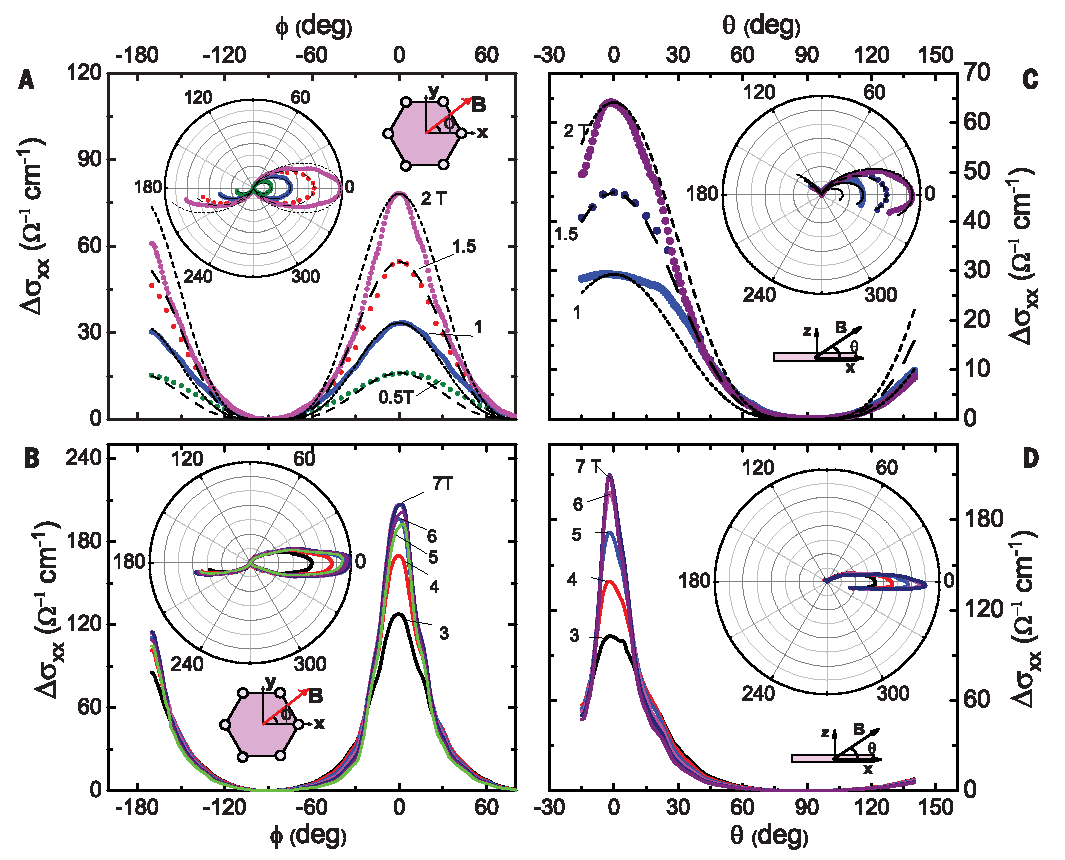
\includegraphics[width=1\linewidth]{ch-na3bi/figures/FigPolar4.pdf}
\caption{\label{figPolar4} 
Angular dependence of the axial current in Sample J4 at 4.5 K inferred from measurements of $R_{14,23}$ in tilted ${\bf B}(\theta,\phi)$. 
In Panels A and B, $\bf B$ lies in the $x$-$y$ plane at an angle $\phi$ to $\bf\hat{x}$ (sketch in insets). The 
conductance enhancement $\Delta \sigma_{xx}$ at fixed $B$ is plotted against $\phi$ for values of $B \le$ 2 T (Panel A) and for $3\le B\le 7$ T (Panel B). Fits to $\cos^4\phi$ (dashed curves), while reasonable below 2 T become very poor as $B$ exceeds 2 T. The insets show the polar representation of $\Delta \sigma_{xx}$ vs. $\phi$. In Panels C and D, $\bf B$ is tilted in the plane $x$-$z$. As sketched in the insets, $\theta$ is the angle between $\bf B$ and $\bf\hat{x}$. Curves of $\Delta \sigma_{xx}$ vs. $\theta$ for $B$ = 1, 1.5 and 2 T are shown in Panel C, while Panel D shows curves for $3\le B\le 7$ T. The axial current is peaked when $\phi\to 0$ (or $\theta\to 0$) with an angular width that narrows significantly as $B$ increases.
}
  \end{center}
\end{figure}

Another interesting part is that the negative MR is very large (as shown in Fig.\ref{figMR4}), which indicates a possible long relaxation time $\tau_a$. It is convenient to analyze the contribution of the axial current in conductance. We convert the resistivity into conductance in Fig. \ref{figMR4}C. When $\bf B$ and $\bf E$ are parallel, $G = 1/R_{35,26}$ follows a parabolic behavior that increases with $B$. The dramatic increase of $G$ indicates a long inter-valley relaxation time for the novel current. We fit Eq. \ref{eq:SS} to the $G$ v.s. $B$ curve at $\phi'=0$ in Fig. \ref{figMR4}C. Using the ratio $\sigma_{\chi}/\sigma_0 = \frac34 (k_F\ell_B)^{-4}.(\tau_v/\tau_{tr})$, where $\sigma_0$ is the Drude conductivity, $\ell_B$ is the magnetic length $\sqrt{\hbar/eB}$ and $\tau_{tr}$ the usual transport lifetime, we find that $\tau_v/\tau_{tr}$ = 40-60 in weak $B$. Such a large ratio between the two types of relaxation time implies that the inter valley relaxation rate $1/\tau_v$ of the novel axial current is anomalously lower than the scattering rate $1/\tau_{tr}$ of the conventional states in zero $B$. However, in the quantum limit, $\tau_v$ is strongly suppressed as $\sim 1/B$ because of the continuous increment in LL degeneracy which makes $\sigma_\chi$ $B$-independent, as discussed above (Fig. \ref{figSdH}C). 

To our knowledge, the matrix element $M$ in $1/\tau_a$ is not well studied despite its importance. Thus our data on Na$_3$Bi can provide a helpful direction for the study of the relaxation process of axial currents. Besides, there is some debate on whether a large node separation $2\delta k_N$ is needed to obtain a long $\tau_a$. In a DSM such as Na$_3$Bi, the Weyl nodes originally occupy the same point in the reciprocal space. But they can be split by a magnetic field. We deduce the separation induced by $\bf B$ in our Na$_3$Bi samples using the estimate of $g^* \sim 20$. We find that $\delta k_N > k_F$ when $B > 12$ T. Interestingly, it was shown\cite{Burkov2015} recently that the ratio $\tau_a/\tau_0$ (in a superlattice model) can be very large even for negligible $\delta k_N$. Ref. \cite{Burkov2015} argues that the axial current relaxation is still hampered by the Berry curvature effects while the chiral symmetry is only weakly violated. This issue should be resolvable by future LMR experiments.

%Then we hope to estimate splitting speed of the Weyl nodes of a DSM in a magnetic field. This information is important because the charge pumping effect in a DSM is based on the prediction that Weyl nodes splitting is generated by breaking time reversal symmetry in the DSM. And the displacement of the Weyl node $\delta K$ from the Dirac node in a DSM is governed by $\delta K= \pm g^*\mu_B B/(\hbar v)$ (we will explain the details later). Assuming $g^*\sim50$ (roughly that in Cd$_3$As$_2$~\cite{Jeon2014}) and $v\sim 2\times 10^5$ m/s, we estimate that the Weyl spheres separate ($\delta K > k_F$) when $B>$ 6 T. This significant displacement is consistent with the steep increase in $\sigma_\chi$ in modest $B$.  




We also notice some interesting features in the high field part of $R_{14,23}$ up to $B$ = 35 T. As displayed in Fig. \ref{figMR4}D, at $H_{k}\sim$ 23 T when $\bf B||\hat{y}$, the slopes of the MR curves experience a sudden change. As $\bf B$ is tilted away from $\bf\hat{y}$ ($\phi\to \; 55^\circ$), the feature at $H_k$ becomes better resolved as a kink. The steep increase in $\rho_{xx}$ above $H_k$ may suggest an electronic instability at large $B$ that opens an energy gap. We also notice that $H_k(\phi)$ is sensitive to the angle $\phi$ as the decrease in $\phi$ below $45^\circ$ rapidly increases $H_k(\phi)$ to above 35 T. However, the negative MR curves close to $\phi = 0$ remain almost unaffected by the instability up to 35 T (the small rising background is from a weak $B_z$ due to a slight misalignment and implies the strong collimation of the axial current). 

The above experimental observation can not be explained by the conventional transport theory, and in our view, provides strong evidence for the chiral anomaly effect in Na$_3$Bi. Compared with the standard MR theory, the most surprising feature is the locking of the negative MR pattern to the $\bf B$ vector in Figs. \ref{figMR4}A and \ref{figMR4}B. The narrow plume feature in Fig. \ref{figPolar4} can not be interpreted as anisotropies in the FS properties ($v$ and $\tau_{tr}$ vs. $\bf k$) by the conventional transport theory, because otherwise the direction of the conductivity extrema should be fixed to certain crystal axes. Nevertheless, our observation is consistent with the theoretical prediction of the chiral anomaly -- the axial current peaks when $\bf E$ is aligned with $\bf B$ even for weak fields. This unusual locking pattern in weak $B$ provides an essential signature of the charge pumping effect between the Weyl nodes, rather than merely the negative LMR. Our experiments also confirm the $B^2$ behavior in the semiclassical weak $B$ and indicate a large ratio between $\tau_v$ and $\tau_{tr}$. In the quantum limit, our data show that the enhancement of the conductance stops as the relaxation rate increases. The narrow angular dependence of the axial current, which is unexpected, may provide further insight into its unusual properties. 







%%%%%%%%%%%%%%%%%%%%%%%%%%%%%%%%%%
%%%%%%%%%%%%%%%%%%%%%%%%%%%%%%%%%%
%%%%%%%%%%%%%%%%%%%%%%%%%%%%%%%%%% FIGURE 




\subsection{Additional Results of the First Sample}

In previous sections, we have discussed our experimental evidence for the chiral anomaly effect in the Dirac semimetal Na$_3$Bi. Our main results above focus on Sample J4. In this section we also present supplemental data from Sample J4, as well as discussing similar results from a second sample J1. We adopt the same notation system as the one in the previous subsection, i.e. $x$-$y$ axes and contact labels defined in the inset in Fig. \ref{figWeyl}C (and reproduced as an inset in Fig. \ref{J4Raw}A). 
\begin{figure}[!htbp]
  \begin{center}
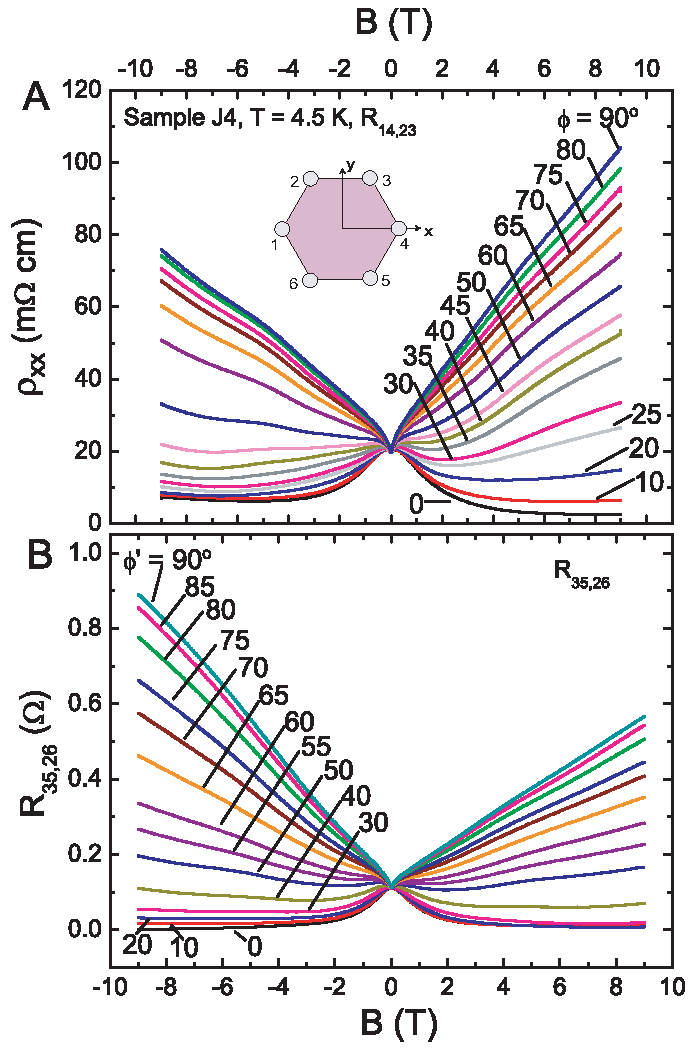
\includegraphics[width=0.75\linewidth]{ch-na3bi/figures/FigJ4RawMR.pdf}
\caption{\label{J4Raw} The unsymmetrized magnetoresistance data in Sample J4. Panel (A): The unsymmetrized MR data at 4.5 K derived from resistance $R_{14,23}$ (current $\bf{I}$ applied to the contacts (1,4) and voltage measured between contacts (2,3)). The inset shows the contact labels and the $x$ and $y$ axes fixed to the crystal. Panel (B): The unsymmetrized MR data based on resistance $R_{35,26}$. The raw data has a small antisymmetric part that we attribute to a small Hall signal inadvertently caused by misalignment between the field tilt plane and the crystal's $a$-$b$ face. Despite this small Hall signal, the negative MR is prominent in both cases when $\phi$ (or $\phi'$) is close to zero.}
  \end{center}
\end{figure}

Many semimetals have a small carrier density $n$ and a high mobility ( e.g. $\mu>$ 20,000 cm$^2$/(Vs)). According to the Drude model, the Hall angle for a one-band metal is $tan \theta_{H} = \mu B$, which increases linearly with the mobility. It indicates that the Hall resistivity $\rho_{yx}$ may become comparable to or even exceed the longitudinal resistivity $\rho_{xx}$. As observed in many of such semimetals, the magnitude of $\rho_{yx}$ indeed greatly exceeds $\rho_{xx}$ (in the standard Hall configuration with current $\bf I||\hat{x}$ and $\bf B||z$). To reduce the influence of the Hall signal, $\bf B$ is aligned to the $x$-$y$ plane as well as possible in most of our experiments. In an ideal case, the Hall effect should be zero when $\bf B$ is parallel to our sample plane. Nevertheless, the experimental data show that  the field-antisymmetric Hall signal is often observed in the background and can be comparable to the resistive voltage above 10 Tesla. One explanation for the mixing is the misalignment of the sample's $a$-$b$ plane to the field rotation plane, thus unintentionally introducing a $z$ component to $\bf B$. Though the misalignment may be small, the remnant $B_z$ could still generate a Hall component that is comparable to $\rho_{xx}$. Since the ideal MR curves are symmetric in field, the mixing of a Hall signal could easily be found from the antisymmetric part of the raw MR curves. Thus a serious misalignment may lead to a large field anti-symmetric distortion in the raw MR curves, making them tilt dramatically towards, say, the $+B$ axis. This mixing effect could be a major source for the observed ``negative resistance'' ($E_{x}<0$ for $\bf I||\hat{x}$) sometimes encountered in semimetal magnetoresistance experiments performed in large $\bf B$. When not treated appropriately, such distortions may imitate a negative MR when the raw curves are symmetrized in field. 

Therefore, to rule out the above possibility of the apparent negative MR caused by Hall mixing, it is important to examine the raw MR curves as well. Here we display the raw MR curves (pre-symmetrization) in Fig. \ref{J4Raw}. They demonstrate that the distortion discussed above is a relatively weak effect in our experiment. When the current $I$ is applied to contacts (1,4) (the measured resistance is $R_{14,23}$), the unsymmetrized raw MR curves measured in Sample J4 are displayed in Figure \ref{J4Raw}A. When $I$ is switched to the contacts (3,5) (measured resistance $R_{35,26}$), the corresponding ``rotated'' curves are exhibited in Figure \ref{J4Raw}B. In Panel A (B), $\phi$ ($\phi'$) denotes the angle between $\bf{B}$ and $\bf\hat{x}$ ($\bf\hat{y}$), following our previously defined notations. Both panels show a small asymmetry in the MR curves, which is caused by a Hall ``pick up'' signal. However, the mixing Hall signal is apparently too small to generate the large, negative MR observed when $\bf B || \bf I$.

\begin{figure}[!htbp]
  \begin{center}
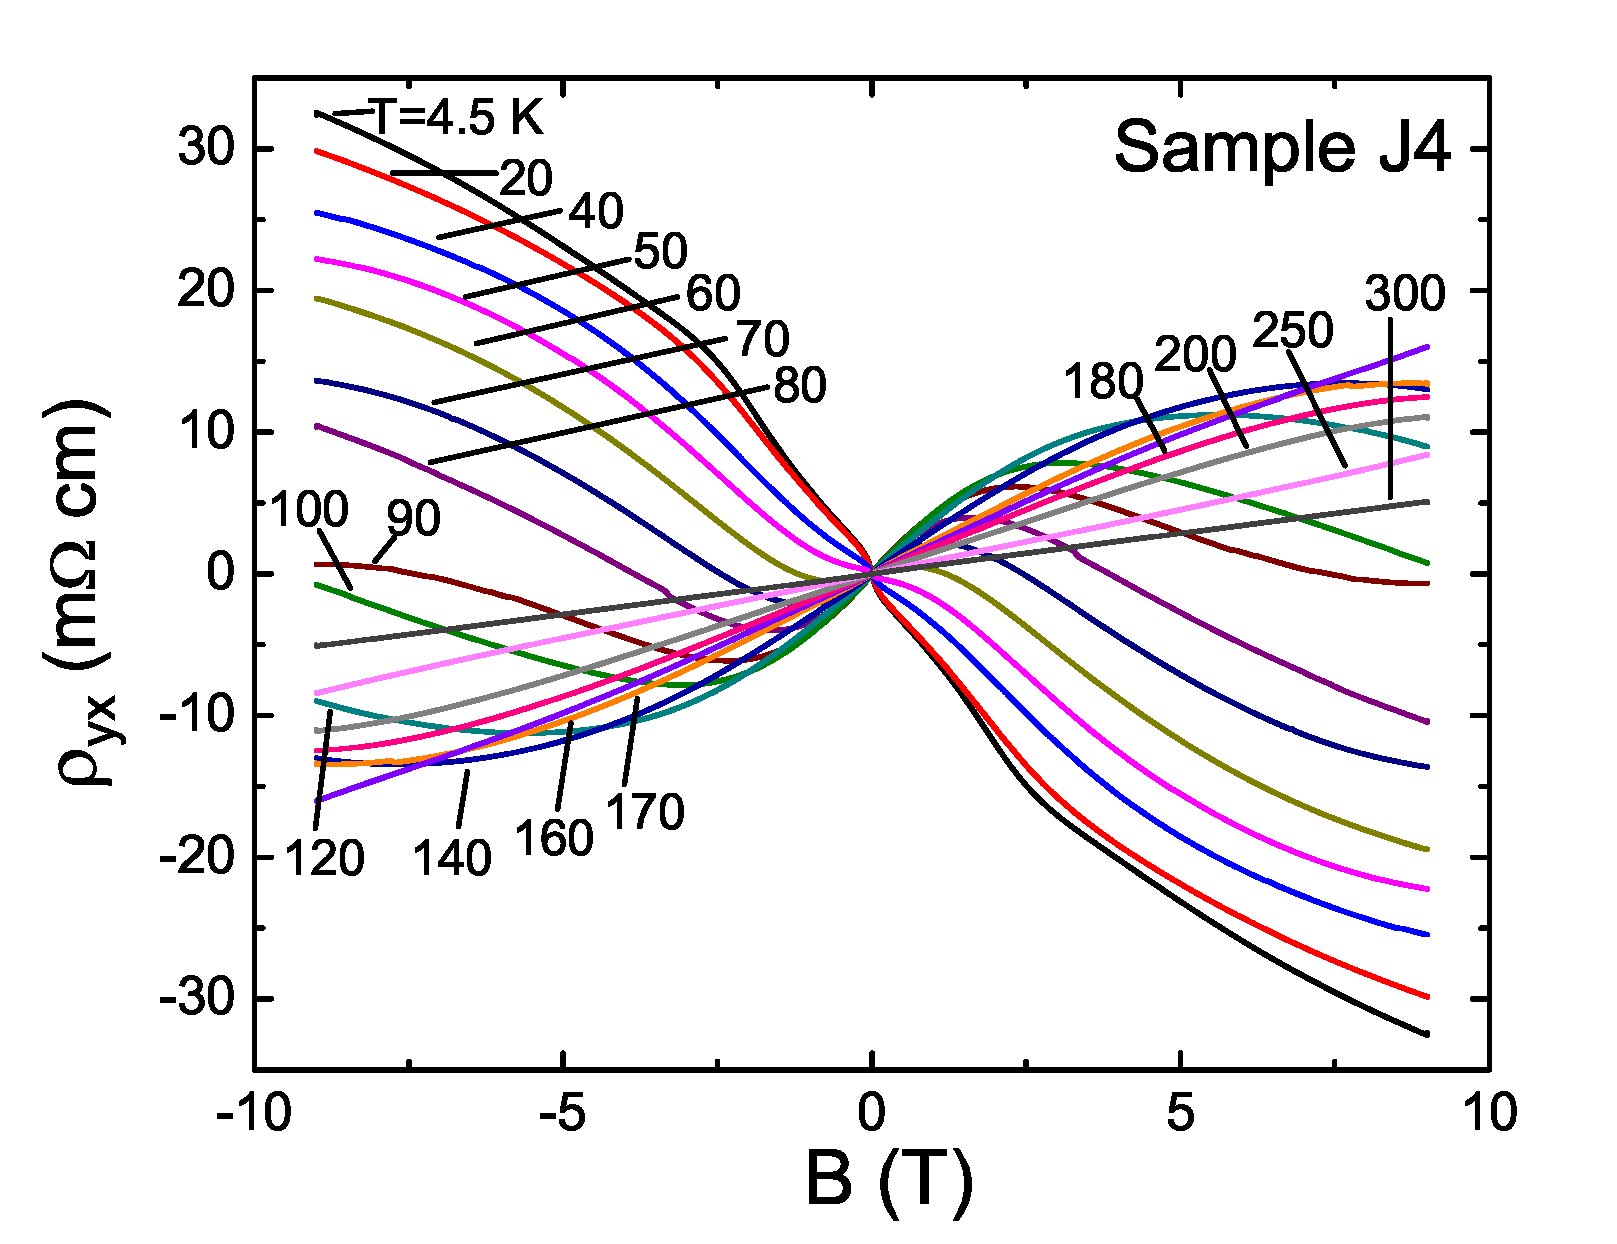
\includegraphics[width=0.8\linewidth]{ch-na3bi/figures/FigJ4Hall.eps}
\caption{\label{J4Hall} The Hall effect data of J4 at different temperatures. The Hall curves at various temperatures reveal a clear signature of thermally excited holes at high temperatures. Above 70 K, the holes start to contribute to the Hall effect and they finally dominate the Hall signal above 140 K. The conductivity enhancement in MR also disappears around the same temperature range.}
  \end{center}
\end{figure}

Figure \ref{J4Hall} shows Hall data at various temperatures in Sample J4, when $I$ is applied to the contacts (1,4) and $\bf{B}$ is parallel to the $c$-axis. The negative slopes at low temperatures indicate electrons' dominance at these temperatures. But when the temperature increases, the hole contribution grows rapidly. The hole contribution could be seen clearly even at a small $\bf{B}$ above 70 K, and it eventually dominates completely above 140 K. This hole excitation behavior is consistent with our estimation of the Fermi energy $\epsilon_F\sim$ 30 mV which is near the Dirac node (Fig. \ref{figWeyl}A). When $T$ is raised above 100 K, the steep increase of both electron and hole densities leads  to the occupation of higher Landau levels (which are not chiral), making the axial current difficult to resolve (Fig. \ref{figWeyl}D).

\begin{figure}[!htbp]
  \begin{center}
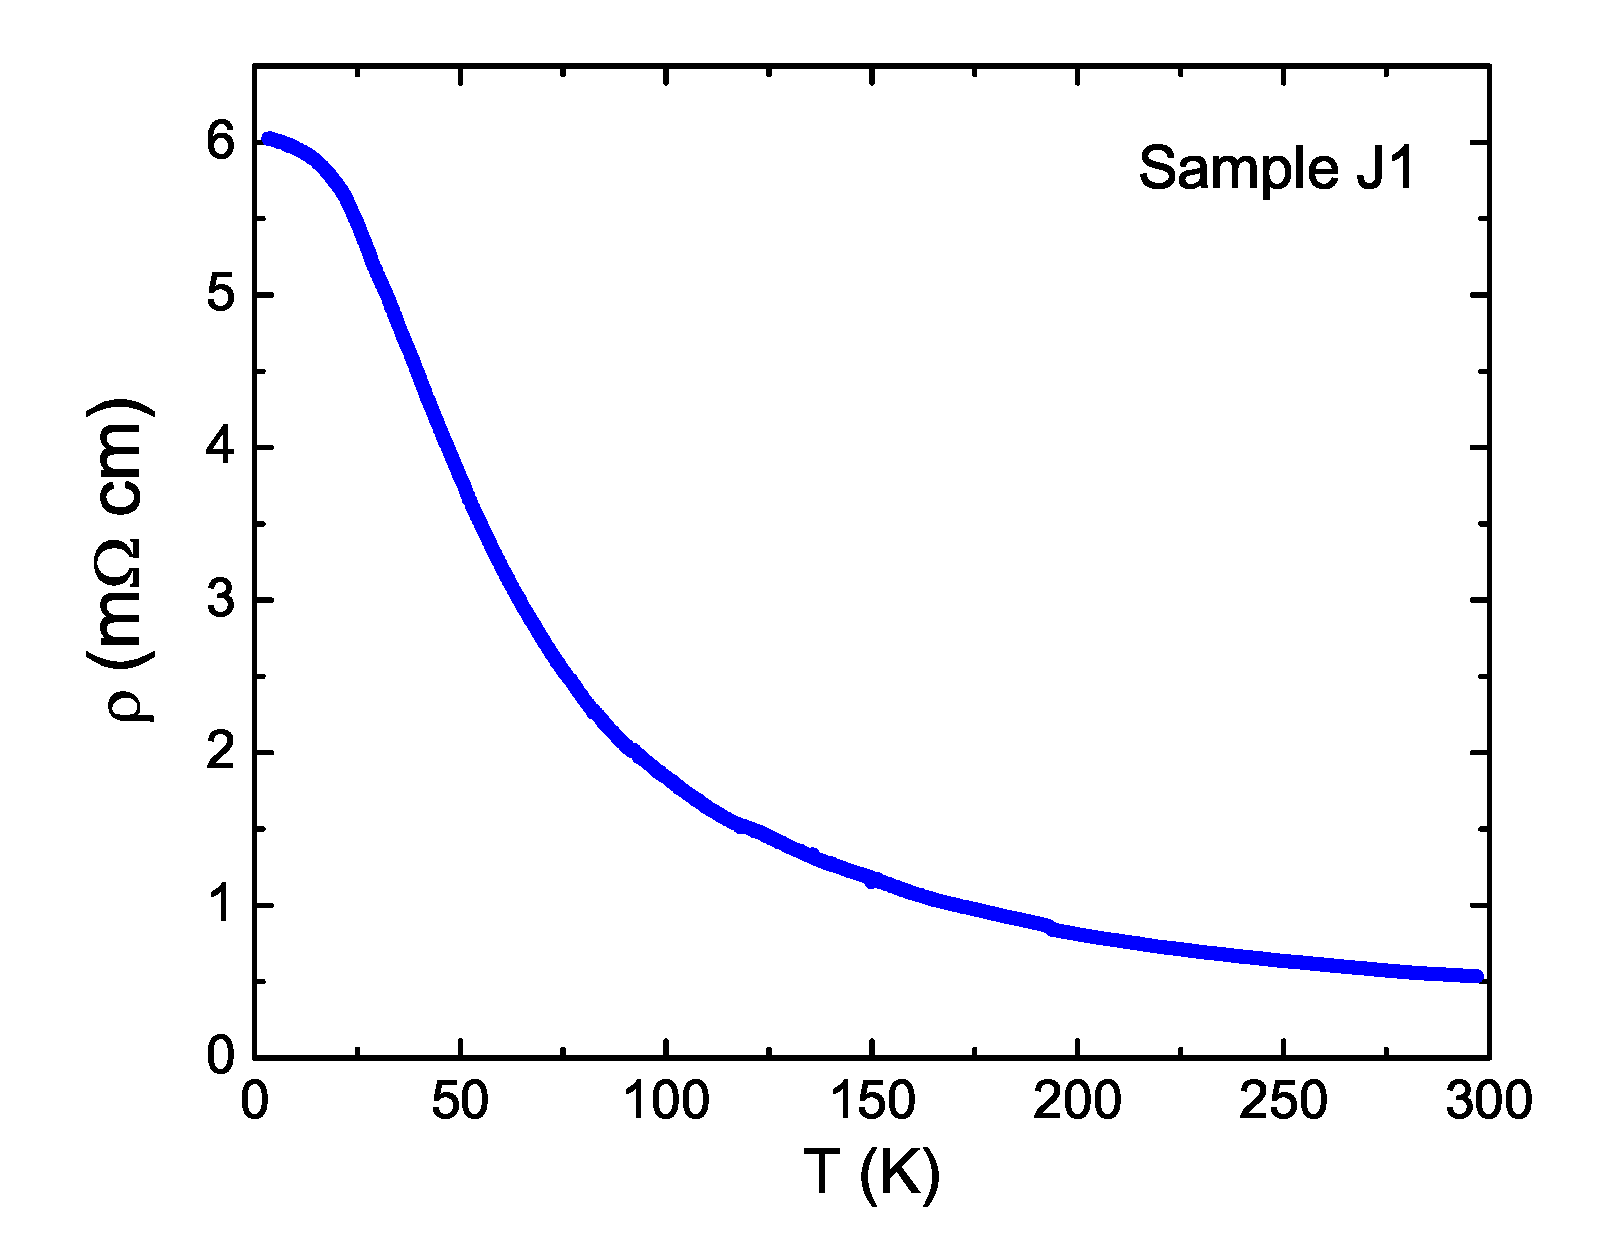
\includegraphics[width=0.75\linewidth]{ch-na3bi/figures/FigJ1rho.eps}
\caption{\label{J1rho} 
Temperature dependence of the resistivity $\rho$ in Sample J1 in zero $B$. The non-metallic profile, closely similar to that in J4, is consistent with
the freezing out of hole excitations as $T\to$ 4 K. 
}
  \end{center}
\end{figure}

\subsection{Negative Longitudinal Magnetoresistance in a Second Sample}
Below we will discuss the transport results on our second sample, J1, which shows behavior similar to that of J4. Both samples were grown within the same boule. Fig.\ref{J1rho} displays J1's non-metallic $\rho-T$ dependence. As in J4, $\rho$ saturates at a peak below 10 K as the hole contribution is frozen out. The value of $\rho$ at 4 K is about 4$\times$ smaller than that in J4. 


The longitudinal magnetoresistance $R_{14,23}$ with $\bf B||\hat{x}$ are shown in Fig. \ref{J1MRT}. When $B$ $<$ 4 T, we observe a large negative MR peak centered at $B$=0 T that gradually disappears when $T$ rises from 3.5 to 120 K. This pattern is similar to the behavior observed in J4, as it hosts a large axial current in the lowest Landau level (LL) which is overwhelmed by contributions from higher LLs at higher $T$. At very large $B$ ($>$ 20 T), the distortion caused by an unintended $z$ component $B_z$ appears in MR curves. 
We measured J1 before J4, and thus we were unaware of the critical alignment conditions needed to isolate the anomalous axial current. Also as no two-axis rotator is available for our field-rotation measurement, the misaligned $z$ component of $\bf B$ might be significant enough to suppress the axial current, even as the field is rotated in the nominal ``$x$-$y$'' plane. 

%%%%%%%%%%%%%%%%%%%%%%%%%%%%%%%%%%
%%%%%%%%%%%%%%%%%%%%%%%%%%%%%%%%%% FIGURE 3
\begin{figure}[!htbp]
  \begin{center}
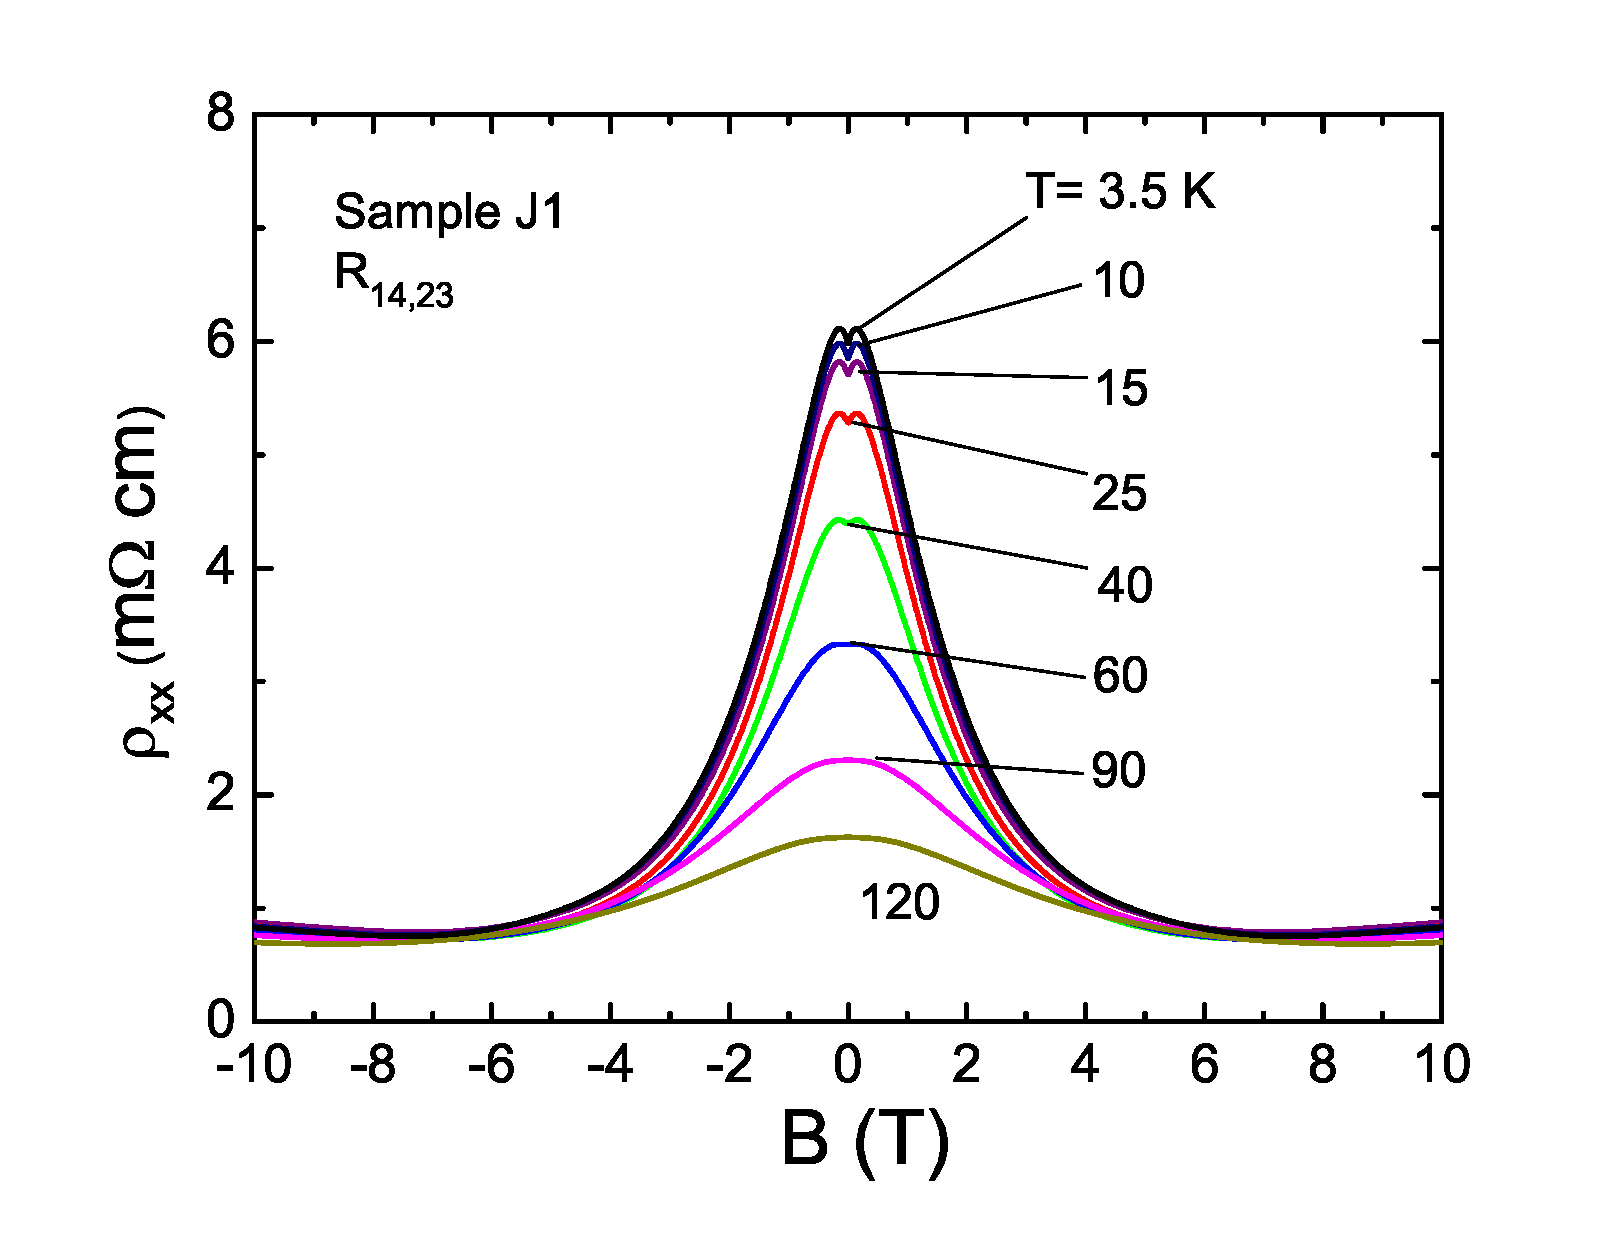
\includegraphics[width=0.9\linewidth]{ch-na3bi/figures/FigJ1MRvsT.eps}
\caption{\label{J1MRT} 
Large negative, longitudinal MR at 3.5 K observed by measuring $R_{14,23}$ with $\bf{B}||\bf\hat{x}$. The negative MR at low fields implies strong increase in the conductance when $\bf{B}||\bf{E}$. As $T$ is raised to 120 K, the negative MR anomaly is progressively suppressed as the conductance of states in upper Landau levels become dominant. The very small increasing background discernible above 7 T reflects a small $B_z$ caused by misalignment.}
  \end{center}
\end{figure}


%%%%%%%%%%%%%%%%%%%%%%%%%%%%%%%%%%
%%%%%%%%%%%%%%%%%%%%%%%%%%%%%%%%%% FIGURE 3




\begin{figure}[!htbp]
  \begin{center}
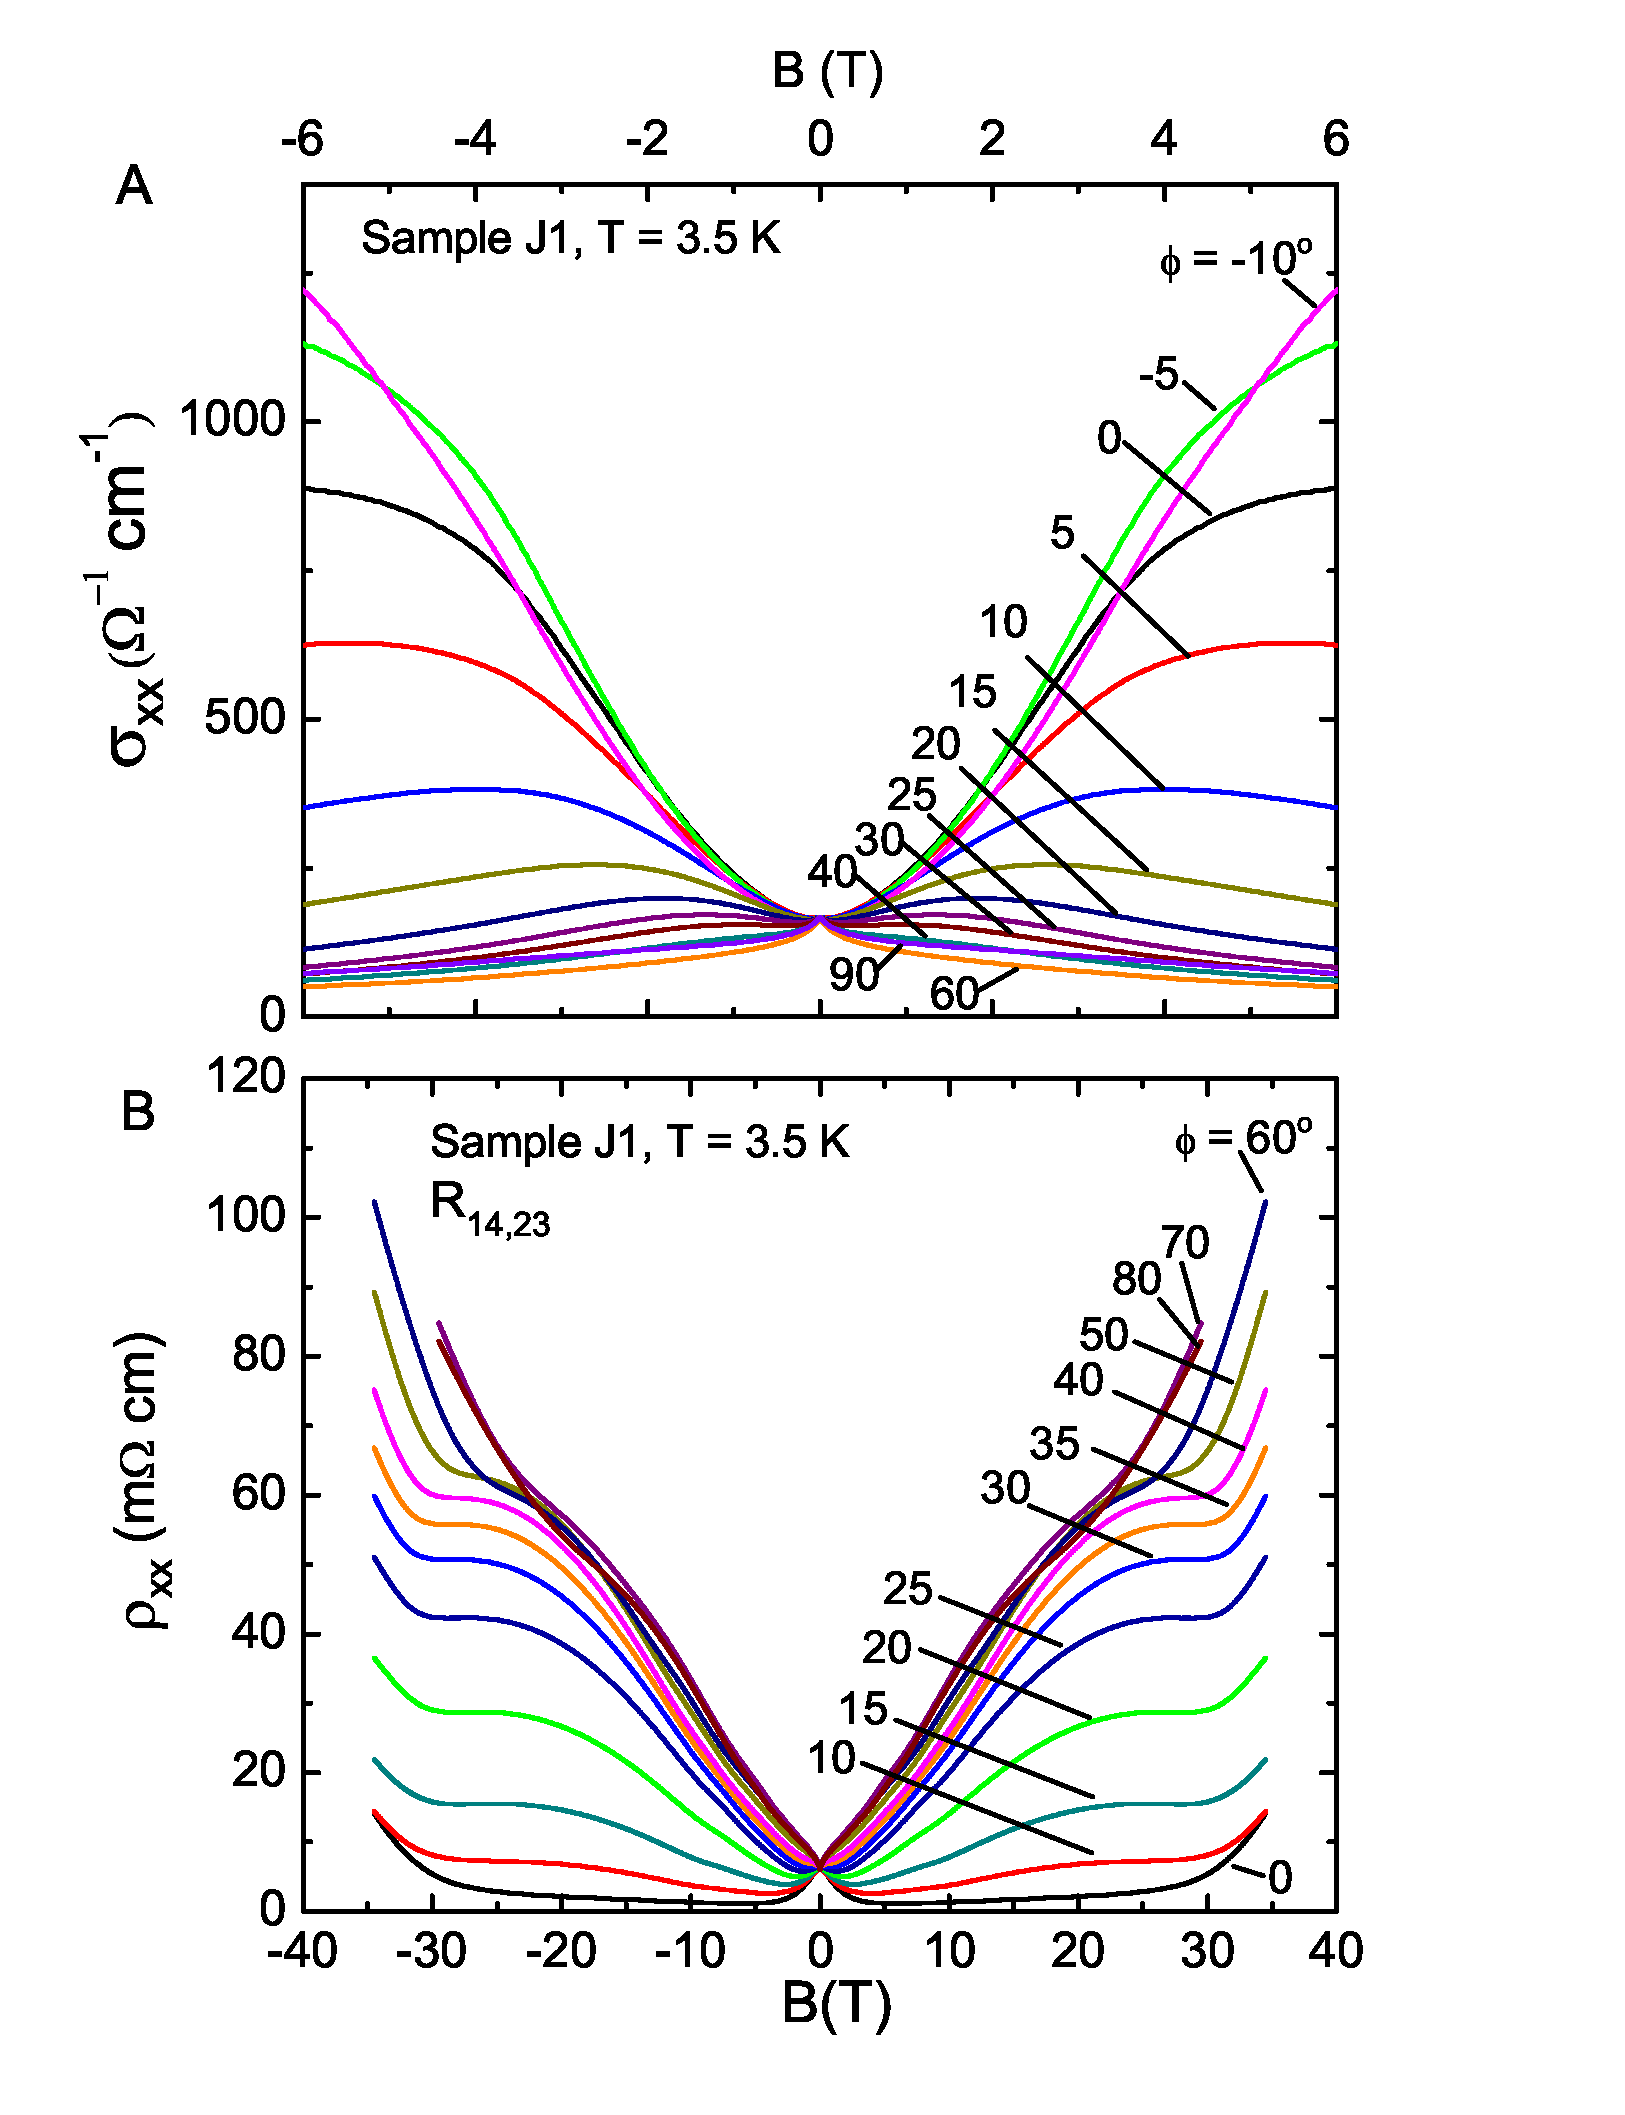
\includegraphics[width=0.8\linewidth]{ch-na3bi/figures/FigJ1CondMR.eps}
\caption{\label{J1MR} Panel (A): Variation of the conductivity curves $\sigma_{xx}(\phi)$ vs. $B$ at selected tilt angles $\phi$ in Sample J1 at $T$ = 3.5 K. 
$\sigma_{xx}(\phi)$ is derived from measurements of $R_{14,23}$. As $\phi$ is rotated to close to 0, $\sigma_{xx}$ increases strongly as $B^2$ consistent with Eq. \ref{eq:SS}. We identify this with the axial current. 
Panel B shows the curves of $\rho_{xx}$ vs. $B$ measured in J1 at 3.5 K at selected tilt angles $\phi$ in fields up to 35 T. The profiles are similar to those shown in Fig. \ref{figMR4}D for Sample J4. A kink feature appears at $H_k$ in the rangle 30-35 T, above which $\rho_{xx}$ increases steeply. Here, the $\phi = 0$ curve (for J1) is also affected by $H_k$ (unlike in J4), possibly because of the larger misalignment in J1.
}
  \end{center}
\end{figure}

Fig. \ref{J1MR}A displays the conductivity $\sigma_{xx}$ v.s. $B$ curves (in J1), which are derived from measurements of $R_{14,23}$, when $\bf B$ is lying in the $x$-$y$ plane (at an angle $\phi$ to $\bf\hat{x}$). As in Sample J4, the conductivity follows a strong $B^2$ enhancement when $\phi$ is close to 0, which is consistent with Eq. 2. Fig. \ref{J1MR}B shows the resistivity $\rho_{xx}$ v.s. $B$ curves measured up to 35 T. Similar to J4, there is a large and positive MR when $\bf B$ is perpendicular to $\bf I$ (curves at 80$^\circ$). But the MR gradually becomes negative as $\phi$ approaches 0$^\circ$. We estimate the misalignment between the $a$-$b$ plane and the field-tilting plane in J1 to be $(10\pm 3)^\circ$. The misalignment has another signature of the misalignment above 30 T. As discussed previously, a knee feature appears at the kink field $H_k\sim$ 30-35 T in Sample J4, above which $\rho_{xx}$ grows rapidly. The $H_k$ of J4 shifts strongly with $\phi$. When $\phi < 25^\circ$ it increases above 35 T (see Fig.\ref{figMR4}D), making the $\phi=0$ curve is unaffected. In Sample J1, we also see a similar kink behavior at high fields. Nevertheless, $H_k(\phi)$ in J1 has a milder dependence on $\phi$ in Fig. \ref{J1MR}B. In particular, a small upturn is observed above 30 T in the 0$^\circ$ curve. We interpret this as an implication of a non-negligible $B_z$ component in the measurement at $\phi$ = 0. 

Therefore, in J1, we have observed the main features of the MR data reported for J4 in the previous section. However, above 30 T, the larger misalignment of the crystal plane in J1 leads to an upturn in $\rho_{xx}$ that does not appear in J4. Comparison of the MR results from J1 and J4 in the large-$B$ limit also implies that angular width of the collimated beam associated with the axial current is narrow. 



%\centerline{*     *     *}\vspace{6in}


\subsection{Resistivity and Conductivity Tensors from Boltzmann Equation in a Tilted Magnetic Field}
In this subsection, we will show that the above MR results of our Na$_3$Bi samples at different directions of $\bf B$ are not expected from the conventional semiclassical, one-band transport theory in a tilted field. Considering a single anisotropic band, the Boltzmann equation that describes the transport pheomena is
\be
e{\bf E\cdot v}\frac{\partial f^0_{\bf k}}{\partial \epsilon_{\bf k}} + e{\bf v\times B}\cdot\frac{\partial g_{\bf k}}{\partial {\bf k}} 
= -\frac{g_{\bf k}}{\tau},
\label{Boltz}
\ee
where $e$ is the electron charge, $\bf E$ is the electric field, $\bf v = \partial\epsilon_{\bf k}/\hbar\partial {\bf k}$ is the Fermi velocity of Bloch electrons, $g_{\bf k}$ is the leading correction to the equilibrium distribution function $f^0_{\bf k}$, and $\tau$ is the relaxation time. We assume that the magnetic field is tilted in the $x$-$z$ plane, i.e. ${\bf B} = (B_1, 0, B_3)$. Using the \emph{ansatz} with $\bf u$ the drift velocity
\be
g_{\bf k} = -{\bf u\cdot k}\frac{\partial f^0_{\bf k}}{\partial \epsilon_{\bf k}},
\ee
and the effective mass matrix
\begin{eqnarray}
\hat{m} = \left[   \begin{array}{ccc}
		m_1   &   0   &   0 \\
		0      &    m_2 &   0 \\
		0     &    0     &   m_3   \end{array}\right]
\end{eqnarray}
we can solve Eq. \ref{Boltz} to obtain the resistivity tensor ($n$ is the carrier density)
\begin{eqnarray}
\hat{\rho} = 
						\left[  	\begin{array}{ccc}
								\rho_1	&  -B_3/ne   &   0  \\
								B_3/ne  &   \rho_2   &   -B_1/ne \\
								0          &   B_1/ne   &   \rho_3   
								\end{array}
								\right].
				\label{rhoij}
				\end{eqnarray}
				

The conductivity tensor can be obtained by inverting $\hat\rho$, which is 
\begin{eqnarray}
\hat{\sigma} = 
						\frac{1}{\Delta}\left[  	\begin{array}{ccc}
								\sigma_1(1+\mu_1\mu_3 B_1^2)  &  \sigma_1\mu_2B_3   &   \sigma_2\mu_1\mu_3 B_1B_3 \\
								 -\sigma_1\mu_2B_3									&   \sigma_2   									&   \sigma_2\mu_3B_1   \\
								\sigma_2\mu_1\mu_3 B_1B_3     &    -\sigma_2\mu_3B_1      &   \sigma_3(1+\mu_1\mu_2B_3^2)
								\end{array}
								\right]
				\label{Sij}
				\end{eqnarray}
where the elements of the conductivity and resistivity tensors at $B$=0 are defined by $\sigma_i = 1/\rho_i = ne\mu_i $. Here the anisotropic
mobilities are $\mu_i = e\tau/m_i$. The determinant $\Delta$ equals $(1+\mu_2\mu_3 B_1^2+ \mu_1\mu_2 B_3^2)$.

The above equations describe how different elements of the conductivity and resistivity tensors will depend on the direction of $\bf B$. An important conclusion is that, despite the anisotropy and the tilted field direction, the longitudinal resistivity 
$\rho_{xx}$ (the three diagonal terms) is strictly independent of $\bf B$, indicating the perfect balance between the Hall E-field and the Lorentz force. In the limit $B_3\to 0$ (or $\theta\to 0$ in Fig. \ref{figPolar4}C,D), the longitudinal conductivity $\sigma_{xx}$ follows a mild field dependence that vanishes if $\mu_1 = \mu_2 = \mu_3$. Therefore, $\sigma_{xx}$ only varies slowly $\theta$, and it never diverges as $1/\sin\theta$ or any other sharp form.

Equations \ref{rhoij} and \ref{Sij} also apply to the configuration with $\bf B$ tilted in the $x$-$y$ plane (Fig. \ref{figMR4} and Fig. \ref{figPolar4}A,B in previous subsections) if we exchange the axes $y\leftrightarrow z$.


\subsection{Splitting of Generated Weyl Nodes of a Dirac Semimetal in a Magnetic Field}
In this subsection, we will discuss a crucial problem of 3D Dirac semimetals, i.e. how much shift can the Weyl nodes have when they are split by a magnetic field . To solve this problem,we leverage the model introduced by Wang \etal~\cite{Wang2012} (see also Jeon \etal~\cite{Jeon2014}), and estimate the shift in the Weyl nodes induced by the magnetic field $\bf B$ as follows. In a field $\bf B\parallel \hat{z}$, we have ${\bf k \to \Pi} = {\bf k} - e{\bf A}$, with the vector potential ${\bf A} = xB{\bf \hat{y}}$. The wavevector $\bf k$ is measured relative to the Dirac node. Neglecting the off-diagonal corrections in the full $4\times4$ Hamiltonian, we can work in the
$2\times2$ matrix of the Hamiltonian for the ``up'' Weyl node with the form 
\begin{eqnarray}
H_+ = \hbar v\left[\begin{array}{cc}
						\Pi_z   &  \Pi_+   \\
						\Pi_-   &   -\Pi_z  
						\end{array}\right]
						-\mu_B B \left[\begin{array}{cc}
						g_s   &   0   \\
						0      &   g_p  
						\end{array}\right],
						\label{H1}
						\end{eqnarray}
where $\Pi_{\pm} = \Pi_x \pm i\Pi_y$ and $\mu_B$ is the Bohr magneton. We can also write the $g$-factors $g_s$ and $g_p$ (which are distinct) of the starting atomic orbitals $|S,\pm\rangle$ and $|P,\pm\rangle$ as $g_s = g_m + \delta g$ and $g_p = g_m - \delta g$. Then the Hamiltonian becomes
\be
H_+ = v{\bf \Pi\cdot }\boldsymbol{\tau} - g_m\mu_B B {\bf 1}- \delta g\mu_B B \tau_3,
\label{H2}
\ee
where $\tau_i$ are the Pauli matrices in orbital space.
To solve it for the energy spectrum, we transform the $\Pi_\pm$ to the raising and lowering operators $a^\dagger$ and $a$, with $\ell_B$ the magnetic length,
\be
\Pi_+ = \frac{\sqrt{2} a^\dagger}{\ell_B}, \quad \Pi_- = \frac{\sqrt{2} a}{\ell_B}
\label{Pi}
\ee
then we diagonalize $H_+$ to obtain the eigenenergy of the $n^{th}$ Landau level
\be
E_n(k_z) = -g_m\mu_B B \pm \sqrt{ \frac{2n\hbar^2 v^2}{\ell_B^2} + (\hbar vk_z -\delta g\mu_BB)^2}.
\label{En}
\ee
To find the splitting of the Weyl nodes, we set the second term under the square root to zero and obtain $\Delta k = \delta g\mu_B B/\hbar v$. Thus the splitting grows linearly with the magnetic field. We also notice that the magnitude of the splitting depends on the difference of the $g$-factors of the two orbits. This is the expression we use in the previous sections to estimate the shift. Consistent with Fig. \ref{figSdH}, the term $-g_m\mu_B B$ in Eq. \ref{En} results in pronounced deviation of the index plot from a straight line if $|g_m|\gg 1$.

\subsection{The Negative MR does not Origin from Localization}

In this subsection, we will demonstrate our evidence that the observed negative LMR cannot be interpreted by localization. Negative MR is not uncommon in the transport experiments of metals. The well-established Anderson localization theory can well explain the negative MR in 2D disordered metals. However, we believe it is irrelevant to the negative LMR in our Na$_3$Bi. We discuss the reasons below.

Here we briefly review the picture of Anderson localization. When electrons diffuse in a disordered metal at very low $T$, the transmission amplitude $\mathcal{A}$ between two points P and P$'$ is the sum of contributions over all Feynman paths linking P to P$'$. We may consider an electron's path that forms a loop and returns to the origin. In a diffusive system, the loop size L is much larger than the electron mean-free-path $\ell$. In this loop, the electron can be scattered by several impurities. An electron can travel clockwise or anticlockwise on the loop, and the two paths form a time-reversal partner for each other. Since these two paths always have the same phase and interfere constructively, their amplitudes are greatly enhanced, especially compared to other random-averaged paths. As a result, the electrons are more likely to be restricted inside these paths and it leads to Anderson localization. Such phenomena are more distinct at lower temperatures when the inelastic scattering with phonons is suppressed. At a high temperature, the phonon scattering destroys the quantum coherence and makes L decrease rapidly. In a 2D system, the weak localization results in the log$T$ increase of the resistance. For 3D metals, $R$ varies as $T^{-n}$ (n = $\frac14$ $\to$ $\frac12$ ).

When a magnetic field is applied, the phases of the clockwise or anticlockwise paths will differ, and it will steeply reduce the constructive interference. Therefore, the MR becomes negative as the localization effect is weakened by $\bf B$. In 2D, $\Delta R$ follows a -log$|B|$ dependence in a low field while it varies as $B^{-\frac12}$ in 3D. In 2D metals, the characteristic field decreases from 100 G at 2 K to 20 G at 100 mK, as $L$ increases. There are many experiments showing the weak localization effect in 2D. Nevertheless, this effect is rare in 3D systems, since the Feynman paths in 3D seldom self-intersect and the quantum correction term is not large.

% Since different paths interfere with each other, some paths almost cancel each other's contribution from P to P$'$ in zero magnetic field. 
%If we invert one of these two paths, we will see that the two paths form a closed loop and the amplitude doubles. Such closed loops indicate that electrons have a lower probability to transmit to other positions and thus become localized. In a modest magnetic field, the phase in the loops are tuned by the magnetic field and the amplitudes of these localized loops decrease. Thus it can cause a negative MR.


%The diffusive nature of electrons moving in a sea of impurities dictates that the size L of a closed loop is generally $\gg$ $\ell$, the electron mean-free-path. In zero $B$, the 2 paths traversing a closed loop (clockwise v.s. anticlockwise) are exact time-reversed partners. Hence
%wave packets following the two paths must interfere constructively when they return to the node regardless of $L$. Consequently, the amplitude for observing the electron at the node is enhanced, leading to Anderson localization. Because raising $T$ increases inelastic scattering by phonons (which destroys the quantum coherence), $L$ shrinks rapidly with increased $T$. As $T$ decreases, the quantum corrections lead to a resistance $R$ that increases as log$T$ in 2D. For 3D metals, $R$ varies as $T^{-n}$ (n = $\frac14$ $\to$ $\frac12$ ). In finite $B$, the constructive interference is suppressed once the magnetic flux in $L^2$ exceeds $\sim$ $\frac12$ a flux quantum $\phi_0$. As noted, this leads to a negative MR,with $\Delta R$ $\sim$ log$B$ in 2D. In 3D,$\Delta R$ $\sim$ $B^{-\frac12}$. In 2D metals, the characteristic field decreases from 100 G at 2 K to 20 G at 100 mK, as $L$ increases. Experimentally, 2D localization has been extensively investigated. In 3D metals, however, it has been difficult to observe in MR experiments. The corrections are weak presumably because Feynman paths in 3D rarely self-intersect.

The following are the reasons why we believe localization is not relevant in our Na$_3$Bi samples:

First, the $\rho$ v.s. $T$ curve in $B$ = 0 (Fig.\ref{figWeyl}C) shows that $\rho$ increases by a factor of $\sim$ 12 when $T$ decreases from 300 K. The large variation $\Delta \rho$ between 30 and 100 K is matched by a large change in $R_H$ as we measured. It indicates that the increase in $\rho$ as $T$ decreases results from the frozen holes across the zero gap in Na$_3$Bi rather than Anderson localization (which should not be observable above a few K in 3D either). The $\rho$ v.s. $T$ curve also saturates to a constant below 25 K, contradicting with the prediction of localization that suggests a continuous and sharp increase of $\rho$ as T $\to$ 0 K. 

Second, the localization effect in a 3D metal is rather isotropic in $\bf B$ while the axial current in Na$_3$Bi has a noticeable angular anisotropy when $\bf B$ tilts. For example, Figs. \ref{figMR4} and \ref{figPolar4} show that the large negative LMR can only be observed when $\bf B$ is aligned to $\bf I$ within 3-5 degrees. The steep suppression of the axial current when $\bf B$ deviates from $\bf E$ cannot be explained by the 3D localization, since the quantum interference in 3D localization is equally reduced by $\bf B$ from different directions. In addition, the negative LMR persists up to 90 K, while the 3D localization effects usually happen below 2 K.

Third, the overall change of $\rho_{xx}$ in the negative MR profile of Na$_3$Bi (Fig. \ref{J1MRT} and Fig. \ref{figWeyl}D of main text) is much larger than that in a typical localization system. $\rho_{xx}$ decreases by a factor $>$ 5 at 4 K in Na$_3$Bi. By contrast, the decrease in a typical 2D localization system is within a few \% while the change is even smaller in 3D case. Also, the field scale $B_{\omega}$ needed to suppress the peak in $\rho_{xx}$ is 3-4 T for Na$_3$Bi, much larger than the $<$100 Oe field that is typical in localization experiments. Furthermore, if the negative MR were indeed induced by the localization, then the typical loop size would be $L = \sqrt{\phi_0/2B_{\omega}} \simeq 25$ nm at 4 K, but such a small L could not produce the pronounced 5$\times$ change in $\rho_{xx}$. Moreover, such a small $L$ implies a very short mean free path $\ell$, inconsistent with the measured mobility ($\mu$ = 2600 cm$^2$/(Vs) at 4 K).
